\documentclass[sn-apa]{sn-jnl}% APA Reference Style 
% \documentclass[sn-apa,iicol]{sn-jnl}% APA Reference Sytle with Double Column

%%%% Standard Packages
%%<additional latex packages if required can be included here>

\usepackage{graphicx}%
\usepackage{multirow}%
\usepackage{amsmath,amssymb,amsfonts}%%%
\usepackage{amsthm}%
\usepackage{mathrsfs}%
\usepackage[title]{appendix}%
\usepackage{xcolor}% shi
\usepackage{textcomp}%
\usepackage{manyfoot}%
\usepackage{booktabs}%
\usepackage{algorithm}%
\usepackage{algorithmicx}%
\usepackage{algpseudocode}%
\usepackage{listings}
\usepackage{rotating}
\usepackage{adjustbox}
\usepackage{booktabs}
\usepackage{longtable}
\usepackage{ltablex}
\usepackage{tabu}
\usepackage{verbatim}
\usepackage{multirow}
\usepackage{enumitem}


%%%% uespackages needed for APA7 style
\usepackage[utf8]{inputenc}
\usepackage[style=apa, backend=biber]{biblatex}
\addbibresource{sn-bibliography.bib}


%% as per the requirement new theorem styles can be included as shown below
\theoremstyle{thmstyleone}%
\newtheorem{theorem}{Theorem}%  meant for continuous numbers
%%\newtheorem{theorem}{Theorem}[section]% meant for sectionwise numbers
%% optional argument [theorem] produces theorem numbering sequence instead of independent numbers for Proposition
\newtheorem{proposition}[theorem]{Proposition}% 
%%\newtheorem{proposition}{Proposition}% to get separate numbers for theorem and proposition etc.

\theoremstyle{thmstyletwo}%
\newtheorem{example}{Example}%
\newtheorem{remark}{Remark}%

\theoremstyle{thmstylethree}%
\newtheorem{definition}{Definition}%

\raggedbottom

%%\unnumbered% uncomment this for unnumbered level heads

\begin{document}

\title[Reliability SPE ]{A Multiverse Assessment of the Reliability of the Perceptual Matching Task as a Measurement of the Self-Prioritization Effect}


\author[1,2]{\fnm{Zheng} \sur{Liu}}
\equalcont{These authors contributed equally to this work.}

\author[1]{\fnm{Mengzhen} \sur{Hu}}
\equalcont{These authors contributed equally to this work.}

\author[1]{\fnm{Yuanrui} \sur{Zheng}}

\author[3]{\fnm{Jie} \sur{Sui}}

\author*[1]{\fnm{Hu} \sur{Chuan-Peng}}\email{hu.chuan-peng@nnu.edu.cn; hcp4715@hotmail.com}

\affil*[1]{\orgdiv{School of Psychology}, \orgname{Nanjing Normal University}, \orgaddress{\city{Nanjing}, \country{China}}}

\affil*[2]{\orgdiv{ School of Humanities and Social Sciences}, \orgname{The Chinese University of Hong Kong-Shenzhen}, \orgaddress{\city{Shenzhen}, \country{China}}}

\affil*[3]{\orgdiv{School of Psychology}, \orgname{University of Aberdeen}, \orgaddress{\city{Old Aberdeen}, \country{Scotland}}}


%%==================================%%
%% sample for unstructured abstract %%
%%==================================%%

\abstract{The Self Perceptual Matching Task (SPMT) is a widely used tool to investigate the cognitive processes underlying the Self-Prioritization Effect (SPE), wherein performance is enhanced for self-associated stimuli compared to other-associated ones. Despite the widely use of SPMT, there is a lack of attention on its reliability assessment. This oversight is concerning, given the prevalence of the reliability paradox in cognitive tasks: although cognitive tasks produce robust experimental effects, they do not demonstrate the same level of reliability when evaluating individual differences. To bridge this gap, this preregistered study investigated the reliability of SPMT using a multiverse approach. Considering the various indicators and baselines used to quantify SPE in SPMT, we examine the reliability of 24 SPE measures across 17 datasets (N = 805). We calculated the Split-Half Reliability (\textit{r}) and Intraclass Correlation Coefficient (ICC2) for each SPE measure. Our findings revealed a robust experimental effect of SPE across datasets. However, when it came to individual differences, SPE measures derived from Reaction Time (RT) and Efficiency exhibited relatively higher, compared to other SPE measures, but still unsatisfied split-half reliability (approximately 0.6). Similarly, for the reliability across multiple time points, as assessed by ICC2, RT and Efficiency demonstrated low levels of test-retest reliability (close to 0.5). These outcomes uncovered the presence of a reliability paradox in the context of SPMT-based SPE assessment. While nearly all the measures of SPE in SPMT displayed robust experimental effects, their reliability were unsatisfying. We discussed the implications of the current study for future studies.}


\keywords{Self-Prioritization Effect (SPE), Self-Perceptual Matching Task (SPMT), Reliability, Multiverse}

\maketitle

\section{Introduction}\label{sec:intro}

The Self-Prioritization Effect (SPE) reflects individuals' biased responses towards self-related information in comparison to information related to others. This phenomenon, documented in 1950s \parencite{cherry1953some}, holding a central position within cognitive psychology and underscoring a core facet of human cognition and self-awareness \parencite{sui2017the}. SPE has been found in a broad range of cognitive tasks \parencite[e.g.,][]{sui2012perceptual,cunningham2008yours, rogers1977self}. Despite SPE is often argued to be a self-specific effect, it has been challenging to be disassociated from familiarity effect. That is, the self-related stimuli, such as own objects, own faces \parencite{keenan2000self,kircher2000towards,turk2002mike}, own voices \parencite{hughes2013i,payne2021perceptual}, or own names \parencite{constable2019it} are usually more familiar to participants than those other-related stimuli. To overcome such limitation, \textcite{sui2012perceptual} introduced the Self Perceptual Matching Task (SPMT), where the self-relatedness (and other-relatedness) was acquired in the lab. In this task, participants first associated geometric shapes with person labels (e.g., circle = you, triangle = best friend, square = stranger) and then performed a matching task, judging whether a shape-label pair presented on the screen match the acquired relationship. A typical pattern from this task is that shapes associated to the self exhibit a processing advantage over shapes related to others. This SPE from SPMT has subsequently been replicated  by many researchers \parencite{constable2019relevant,golubickis2020parts,golubickis2017self,hu2020good}, highlighting the robustness of the effect. 

The reliability of SPMT as a measurement of SPE, however, has not been examined. Here, reliability of a cognitive tasks refers to its consistency and dependability in producing consistent results for the same person across sessions or times \parencite{parsons2019psychological,zorowitz2023}. One common method to assess reliability is the Split-Half Reliability  (\textit{r}), where a test is divided into two halves, and the correlation between the data from these two halves is calculated. A high correlation suggests that the test is internally consistent and measures the same construct reliably \parencite{pronk2022methods}. Another widely used method is the Test-retest reliability, which refers to the extent to which a measurement or assessment tool produces consistent and stable results over time when administered to the same group of individuals under identical conditions \parencite{kline2015handbook}. Both methods are from classical test theory in psychometrics \parencite{borsboom2005measuring}, but they are less known to experimental psychologists. In experimental research, researchers focus on the robustness of experimental effects. Robustness, in this context, pertains to the extent to which a cognitive task consistently produces the same effect at the group level across various independent participant samples. For example, the ``group effect" in the Stop-Signal Task refer to differences in Reaction time between different stop signal delays \parencite{hedge2018reliability}. An effect is considered robust if these differences can be consistently observed in different samples performing the Stop-Signal Task.

In recent years, driven by a growing interest in employing cognitive tasks to assess individual differences, researchers have turned their attention to evaluating the reliability of cognitive tasks \parencite[e.g.,][]{karvelis2023individual,kucina2023calibration}. However, existing findings have raised concerns about the reliability of many cognitive tasks \parencite{hedge2018reliability, rouder2019psychometrics}, with a  considerable body of research highlighting the moderate to low level reliability found in the cognitive task measurements \parencite{clark2022test,green2016use,enkavi2019large}. For instance, \textcite{hedge2018reliability} reported a range of test-retest reliabilities pertaining to frequently employed experimental task metrics (such as Stroop and Stop-Signal Task), with a notable prevalence of discrepancy between the low reliability for individual differences and the robustness of the experimental effects. This discrepancy, named as the ``reliability paradox" \parencite{logie1996group}, has gain much attention in recent years. Like other cognitive tasks, SPMT was also employed by researchers as a measure of individual differences in SPE. For example, a recent study examined the individual difference of SPE and how these individual differences are correlated to brain network \parencite{zhang2023decoding}. Likewise, in clinical investigation, the SPMT has been incorporated to assess deviations in self-processing among specific populations, including individuals affected by autism or depression \parencite{hobbs2023self, liu2022depression}. This trend calls for assessing the reliability of SPMT as a measurement of SPE. 

Further, the variability in quantifying SPE using SPMT calls for a comprehensive examination of the reliability of different SPE measures. As simple as the SPMT, there are multiple approaches to quantify the SPE, encompassing various indicators and baselines. In a typical SPMT experiment, two direct outcomes are generated: Reaction Time (RT) and choices. The RT and Accuracy (ACC) of choices are two most widely used indicators of SPE. Several other indicators can be derived from these direct outcomes:  Efficiency ($\eta$) \parencite{humphreys2015the,stoeber2008perfectionism}, sensitivity score (\textit{d}-prime) of Signal Detection Theory \parencite{hu2020good,sui2012perceptual}, drift rate (\textit{v}) and starting point (\textit{z}) estimated using the Drift-Diffusion Model (DDM) \parencite{golubickis2017self}.  In addition to the variability of indicators, SPE can be estimated by calculating the difference between self condition and different baselines. Indeed, the selection of baselines varies across studies, such as ``Close other” (e.g., Friend) \parencite{navon2021are, svensson2022more}, ``Stranger” \parencite{constable2021affective, orellana2020does}, “Celebrity” (e.g., ``LuXun”) \parencite{qian2020prioritised} and ``Non-person” (e.g., None) \parencite{schafer2019understanding}. As a result, three pivotal questions regarding the reliability of the SPMT remain unresolved: First, given the variability of indicators (RT, ACC, $d'$, $\eta$, \textit{v}, \textit{z}) and choice of baseline conditions (``Close other”, ``Stranger”, ``Celebrity”, and ``Non-person”), which way of quantifying SPE is the most reliable one(s)? Second, is the SPMT suitable for assessing individual differences of SPE? Finally, is there a reliability paradox in the assessment of SPE using SPMT? Addressing these questions is crucial for establishing the formal reliability analysis of SPMT measurements, allowing for accurate assessment of the SPE and its applications in various domains. 

To address these three questions, the present study adopted a multiverse approach to investigate the reliability of SPE measures computed using different indicators under various baseline conditions in the SPMT. This was achieved by re-analyzed 17 independent datasets (N = 805) from 9 papers and 2 unpublished projects that employees SPMT. In order to comprehensively assess the SPE measures derived from SPMT, we created a ``multiverse" of possible indicators (RT, ACC, \textit{d}-prime, $d'$, \textit{v}, \textit{z}) combined with various baseline conditions (``Close other”, ``Stranger”, ``Celebrity”, and ``Non-person”). We first assessed the experimental effect across this multiverse using meta-analysis. The individual level consistency was examined using permutation-based Split-Half Reliability (\textit{r}) and Intraclass Correlation Coefficient (ICC2, Two-way random effect model) for assessing the consistency of task performance over time. The findings of our study provided valuable insights into the reliability of SPMT and its indicators, having the potential to facilitate the future utilization of SPMT in research, clinical settings, and personal performance monitoring.

\section{Methods}\label{sec:method}

\subsection{Ethics Information}\label{subsec:ethics}

As this study is a secondary analysis of pre-existing data sourced from publicly available datasets or archived data previously collected by the author's group, informed consent and confidentiality are not applicable.

\subsection{Experimental Design}\label{subsec:experimentdesign}

Here we provided a detailed overview of the original experimental design of SPMT, as described in the Experiment 1 by \textcite{sui2012perceptual}. The original SPMT used a 2 by 3 within-subject design. The first independent variable, labeled ``Matching,” consisted of two levels: ``Matching” and ``Non-matching”, indicating whether the shape and label were congruent. The second independent variable, labeled ``Identity”, comprised three levels: ``Self”, ``Friend”, and ``Stranger”, representing the corresponding identity associated with the shape.

The original SPMT consisted two stages (refer to Fig. \ref{fig:SPMT_procedure}). In the first stage (instructional stage), participants were instructed to associate three geometric shapes (circle, triangle and square) with three labels (self, friend, and stranger) for approximately 60 seconds. The shape-label associations were counter-balanced between participants. In the second phase (matching task), participants completed a perceptual matching task. Each trial started with a fixation cross displayed in the center of the screen for 500 ms, followed by a shape-label pairing and fixation cross for 100 ms. the screen then went blank for 1500 ms, or until a response was made. Participants were required to judge whether the presented shape and label matched the learned associations from the learning phase and respond as quickly and accurately as possible by pressing one of two buttons within the allowed timeframe. Prior to the formal experimental phase, participants completed a training session consisting of 24 practice trials. After the training, participants completed six blocks of 60 trials in the matching task, with two matching types (matching/non-matching) and three shape associations, for a total of 60 trials per association. Short breaks lasting up to 60 seconds were provided after each block.
 

\begin{figure}[!htbp]
	\centering
	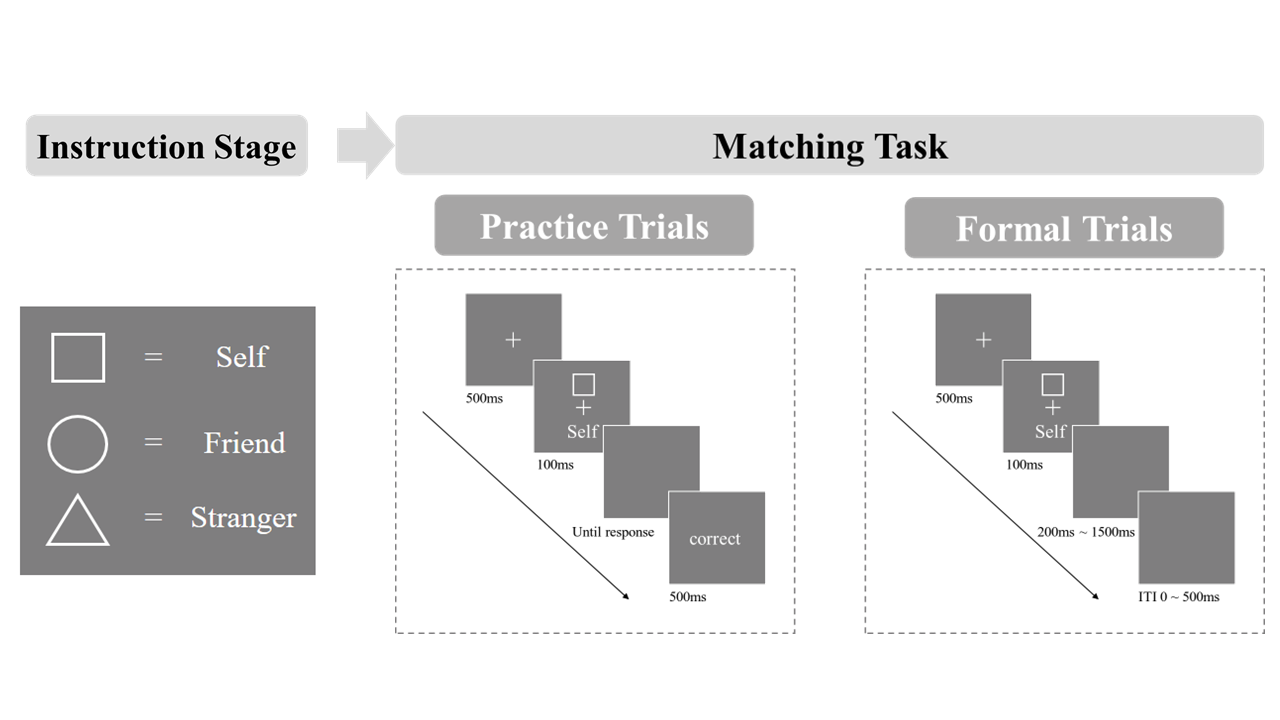
\includegraphics[width=0.9\textwidth]{./Figure/Fig_1_exp_pro.png}
	\caption{Procedure of the original SPMT in Experiment 1 \parencite{sui2012perceptual}. \textit{Note}: The relation between shape-label pairs was counter-balanced between participants.
	}\label{fig:SPMT_procedure}
\end{figure}

\subsection{Datasets Acquisition}\label{subsec:dataset}

Initially, two datasets that employed the SPMT were available to us: one from an unpublished project conducted in our laboratory \parencite{hu2023data}, for which we provide more details in the supplementary materials (section 1.1), and the other provided by our collaborators \parencite{liu2023to}. Concurrently, we are conducting a meta-analysis on SPE using the SPMT (pre-registration available at OSF (\url{https://osf.io/euqmf})). During this process, we identified an additional 13 papers with datasets potentially suitable for our present study. The selection of these papers was based on specific criteria:

\begin{enumerate}[label=\arabic*)]
	\item The paper must primarily utilize the SPMT as their method.
	\item The experimental design should not incorporate any stimuli that could potentially trigger a familiarity effect (e.g., using self-face, self-name).
	\item The trial-level data is either openly available or declared to be obtainable upon request, enabling us to estimate at least one reliability index.
\end{enumerate}


Among the 13 papers included, 7 papers made their trial-level data publicly available \parencite{constable2021affective,constable2020sticking,golubickis2021judging,navon2021are,qian2020prioritised,schafer2019understanding,svensson2022more}. For the remaining 6 papers, we reached out to the authors and requested access to their trial-level data. Out of those 6 requests, 3 papers provided us with trial level data \parencite{kolvoort2020temporal,wozniak2018prioritization,xu2021romantic}. However, in one article, the author did not provide the explanation of the shape and label in the original data \parencite{kolvoort2020temporal}. As a result, we were unable to analyze the raw data in this context. Two papers provided us only with descriptive results \parencite{cheng2019saliency,martinez2020examining}, which unfortunately could not be used for calculating reliability. Additionally, one paper referred to data being shared on the Open Science Framework (OSF) platform \url{https://osf.io/pcv3u/}) \parencite{bukowski2021socio}, but we found that the repository was empty, making it ineligible for the current analysis. 

In total, our analysis comprised raw data from 9 papers and 2 unpublished projects from our laboratory and collaborators. It is important to highlight that the research culture discourages direct replications \parencite{makel2012replications}. As a result, all the datasets included in our analysis underwent some degrees of modification to the original design (e.g., change shapes, modify sequence) as well as including additional independent variables (refer to Table \ref{table:dataset} for specification). For our analysis, we focused exclusively on datasets that adhered to the original design of SPMT without incorporating any stimuli that could potentially trigger a familiarity effect. For datasets from experiments that manipulated other independent variables (e.g., mood), we only utilized data from control conditions so that the data were close to the original design of SPMT. In the end, we were able to incorporate 17 independent datasets from the above-mentioned papers and projects. Nonetheless, not all studies incorporated retest sessions. If a publicly available datasets did not include retest session with SPMT, we excluded it from calculating the Intraclass Correlation Coefficient and only considered the split-half reliability. The details of the included studies and conditions in the datasets are described in Table \ref{table:dataset}. 
\clearpage
\begin{sidewaystable}[!ht]
	\tiny
	\caption{Datasets Information}\label{table:dataset}
	\begin{tabular*}{\textwidth}{@{\extracolsep\fill}lp{0.5cm}p{1cm}p{1cm}p{1cm}cp{1cm}cccccccccc}
		\toprule%
		&  & \multicolumn{4}{@{}c@{}}{Independent Variable} & & & \multicolumn{6}{@{}c@{}}{SPE Indices} & \multicolumn{2}{@{}c@{}}{Reliability}\\\cmidrule{3-6}\cmidrule{9-14}\cmidrule{15-16}%
		Author \& Publication Year & Study & IV 1 & IV 2\centering & IV 3\centering & IV 4 & Sample Size & \begin{tabular}[c]{@{}c@{}}
			\# of Trials\\ per Condition
		\end{tabular} & RT & ACC & $d'$ & $\eta$ & \emph{v} & \emph{z} & ICC & SHR \\
		\midrule
		\textcite{hu2023data} & 1 & Matching & Identity\centering & 
		Emotion \textbf{Control}, Neutral, Happy, Sad\centering & Session\textbf{ 1-6} & 33 & 60 & $\surd$ & $\surd$ & $\surd$ & $\surd$  & $\surd$ & $\surd$ & $\surd$ & $\surd$ \\
		\textcite{constable2020sticking} & 1 & Matching & Identity\centering & 
		Switch Identity Partner, Stranger\centering & Phase \textbf{1}-2& 92 & 40 & $\surd$ & $\surd$ & $\surd$ & $\surd$  & $\surd$ & $\surd$ & & $\surd$ \\
		\textcite{constable2021affective} & 2 & Matching & Identity  Self; Stranger\centering & $--$\centering & $--$ & 56 & 24 & $\surd$ & $\surd$ & $\surd$ & $\surd$  & $\surd$ & $\surd$ & & $\surd$\\
		\textcite{qian2020prioritised} & 1 & Matching & Identity Self; Stranger; Celebrity\centering & Cue With, \textbf{Without}\centering & $--$ & 25 & 24 & $\surd$ & $\surd$ & $\surd$ & $\surd$  & $\surd$ & $\surd$ & & $\surd$ \\
		& 2 & Matching & Identity Self; Celebrity\centering & Cue With, \textbf{Without}\centering & $--$ & 32 & 50 & $\surd$ & $\surd$ & $\surd$ & $\surd$  & $\surd$ & $\surd$ & & $\surd$ \\
		\textcite{schafer2019understanding} & 1 & Matching & Identity Self, Mother, Acquaintance\centering & $--$\centering & $--$ & 35 & 24 & $\surd$ & $\surd$ & $\surd$ & $\surd$  & $\surd$ & $\surd$ & & $\surd$ \\
		\textcite{golubickis2021judging} & 1 & Matching & Identity\centering & Presentation \textbf{Mixed}; Blocked\centering & $--$ & 30 & 30 & $\surd$ & $\surd$ & $\surd$ & $\surd$  & $\surd$ & $\surd$ & & $\surd$ \\
		 \textcite{navon2021are} & 1 & Matching & Identity\centering & $--$\centering & $--$ & 13 & 60 & $\surd$ & $\surd$ & $\surd$ & $\surd$  & $\surd$ & $\surd$ & & $\surd$ \\
		 & 3 & Matching & Identity Self; Father; Stranger\centering & $--$\centering & $--$ & 28 & 60 & $\surd$ & $\surd$ & $\surd$ & $\surd$  & $\surd$ & $\surd$ & & $\surd$ \\
		& 4 & Matching & Identity\centering & $--$\centering & $--$ & 27 & 60 & $\surd$ & $\surd$ & $\surd$ & $\surd$  & $\surd$ & $\surd$ & & $\surd$ \\
		\textcite{svensson2022more} & 1 & Matching & Identity Self; Friend\centering & $--$\centering & $--$ & 20 & 50 & $\surd$ & $\surd$ & $\surd$ & $\surd$  & $\surd$ & $\surd$ & & $\surd$ \\
		& 2 & Matching & Identity Self; Friend\centering & Frequency \underline{Self $>$ Friend}\centering  & $--$ & 24 & 100 & $\surd$ & $\surd$ & $\surd$ & $\surd$  & $\surd$ & $\surd$ & & $\surd$ \\
		& 3 & Matching & Identity Self; Friend\centering & Frequency \underline{Self $<$ Friend}\centering & $--$ & 25 & 100 & $\surd$ & $\surd$ & $\surd$ & $\surd$  & $\surd$ & $\surd$ & & $\surd$ \\
		\textcite{xu2021romantic} & 1 & Matching & Identity\centering & Tasks Modified; \textbf{Unmodified}\centering & $--$ & 105 & 60 & $\surd$ & $\surd$ & $\surd$ & $\surd$  & $\surd$ & $\surd$ & & $\surd$ \\ 
		\textcite{wozniak2018prioritization} & 1 & Matching & Identity\centering & Facial Gender \underline{Male; Female}\centering & $--$ & 18 & 56 & $\surd$ & $\surd$ & $\surd$ & $\surd$  & $\surd$ & $\surd$ & & $\surd$ \\
		& 2 & Matching & Identity\centering & Facial Gender \underline{Male; Female}\centering & $--$ & 18 & 60 & $\surd$ & $\surd$ & $\surd$ & $\surd$  & $\surd$ & $\surd$ & & $\surd$ \\  
		\textcite{liu2023to} & 1 & Matching & Identity Self; Stranger\centering & $--$\centering & $--$ & 298 & 16 & $\surd$ & $\surd$ & $\surd$ & $\surd$  & $\surd$ & $\surd$ & & $\surd$ \\
		\botrule
	\end{tabular*}
	\footnotetext{Study represents different studies from a single article; IV: independent variable. For IV3 and IV4, we only included the baseline conditions that are similar to the original design in \textcite{sui2012perceptual}, which were highlighted in \textbf{BOLD} font. If other variables that could be counterbalanced are indicated by \underline{underscores}, we will solely utilize these variables as stratification variables during the split-half process}
\end{sidewaystable}
\clearpage

\subsection{Analysis }\label{subsec:analysis}

Analysis plans for this study were preregistered on OSF (\url{https://osf.io/pcv3u/}). All analyses in this paper were performed using the statistical software R \parencite{Rcore2021}. The drift rate (\textit{v}) and starting point (\textit{z}) of the Drift-Diffusion Model (DDM) was obtained using the ``RWiener” package \parencite{wabersich2014rwiener}.

The road map of the current study's road-map can be found in Fig. \ref{fig:roadmap} and will be further elucidated in the subsequent sections. 

\begin{figure}[!htbp]
	\centering
	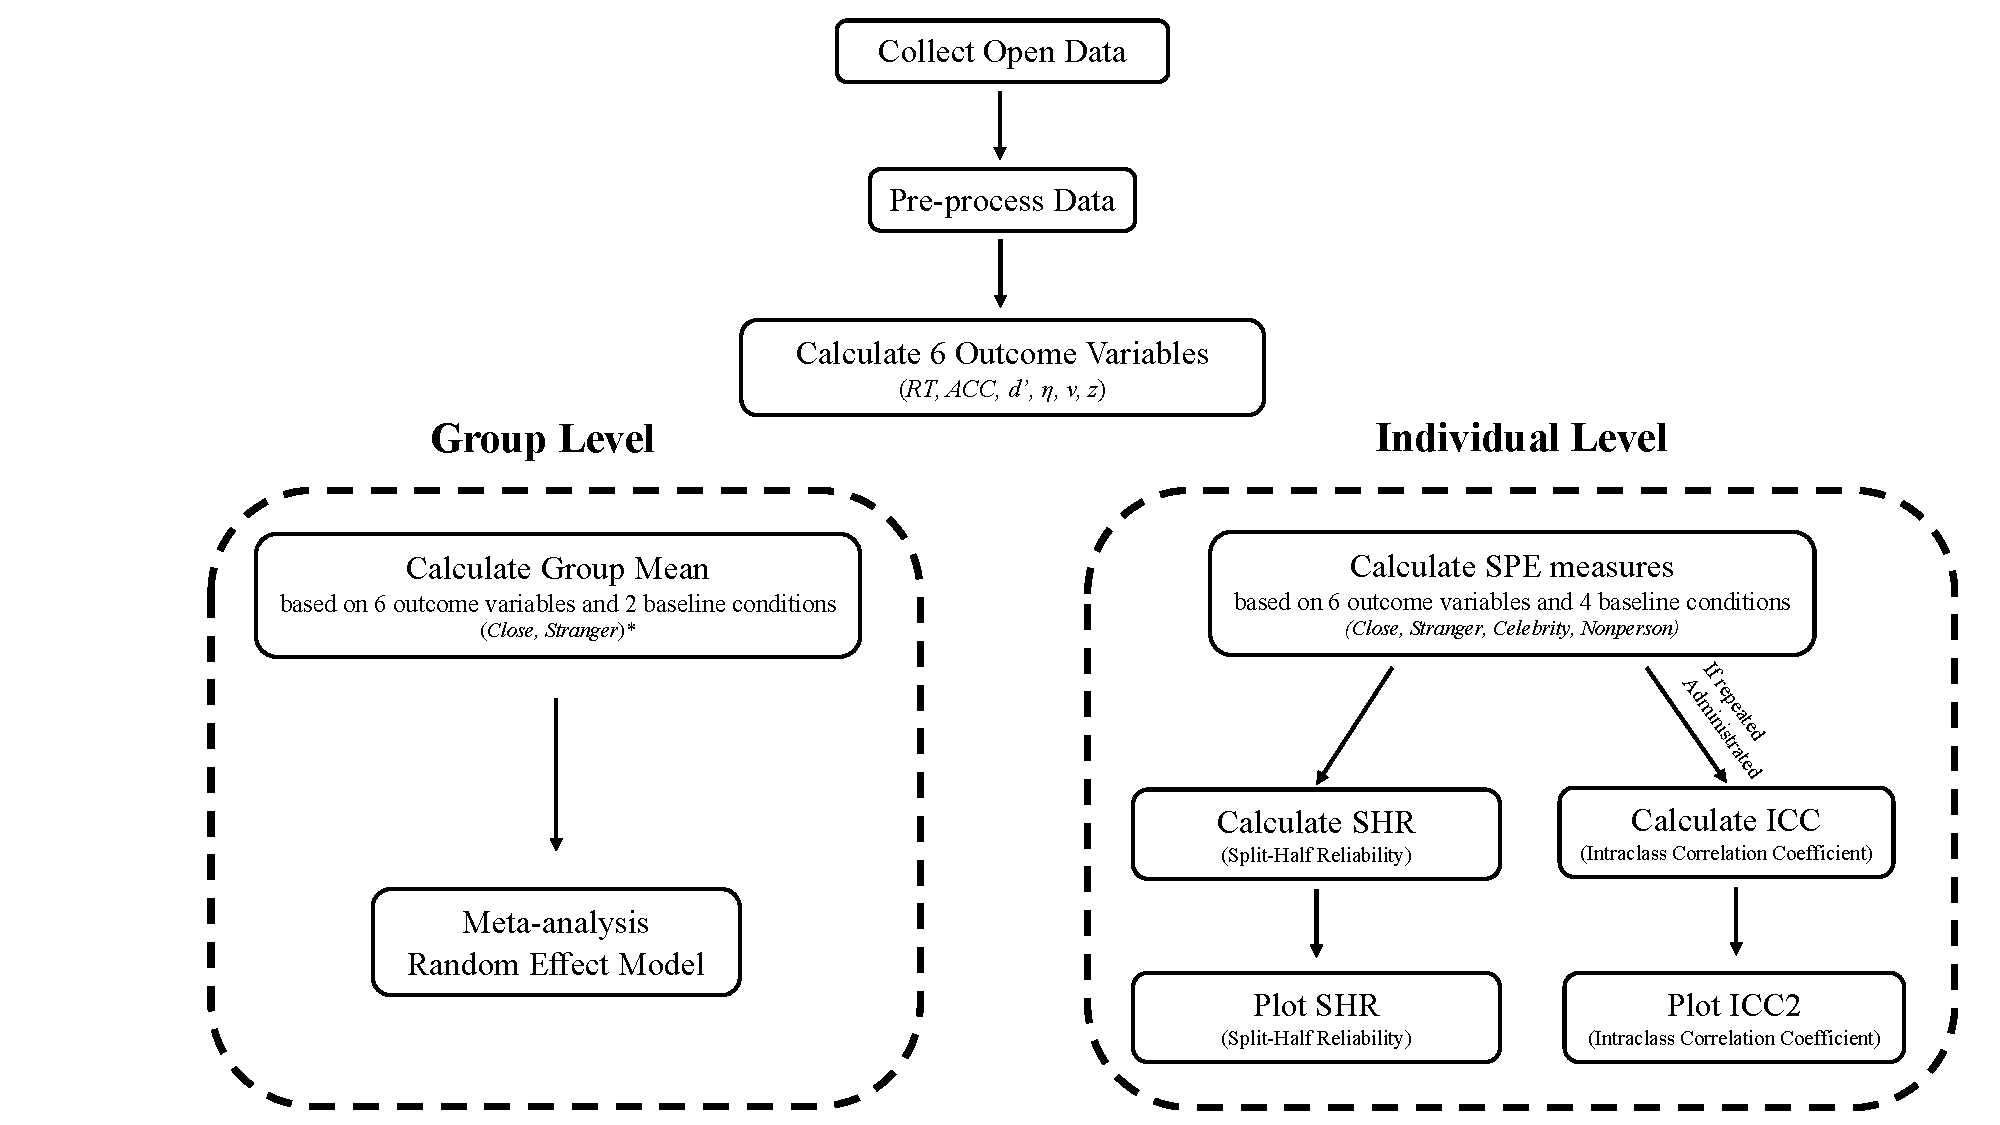
\includegraphics[width=1\textwidth]{./Figure/Fig_2_flow_chart.pdf}
	\caption{Roadmap of the current study. \textit{Note}: Only one paper have Celebrity and Nonpersons baseline, thus no included in the meta-analysis
	}
	\label{fig:roadmap}
\end{figure}

\textbf{\subsubsection{Data Pre-processing }\label{subsubsec:Preprocess}}

For all the seventeen datasets (see Table. \ref{table:dataset}), we applied the following exclusion criteria for excluding data:

\begin{enumerate}
	\item Participant Exclusion Criteria
	
	(\romannumeral1)~Participants who had wrong trial numbers because of procedure errors is excluded from the analysis, 
	
	(\romannumeral2)~participants with an overall accuracy $< 0.5$ is excluded from the analysis, 
	
	(\romannumeral3)~participants with any of the conditions with zero accuracy is excluded from the analysis.
	
	\item Trial Level Data Exclusion Criteria
	
	(\romannumeral1)~ Trials where the keypress occurs outside the two required keys and non-responsive trials are excluded from the analysis, 

	(\romannumeral2)~the practice trials are excluded,
	
	(\romannumeral3)~the experimental design involved independent variables more than self-referential and matching, e.g., included valence of emotion as a third independent variable. 
\end{enumerate}

\textbf{\subsubsection{Calculating the Indicators and SPE Measures }\label{subsubsec:cal_indicies}}

We created a ``multiverse" of SPE Measures. Specifically, for each study, we first calculated six indicators for each experimental condition: Reaction Time (RT), Accuracy (ACC), Sensitivity Score ($d'$), Efficiency ($\eta$), Drift Rate (\textit{v}), and Starting Point (\textit{z}). Reaction Time and Accuracy were obtained directly from the datasets, while sensitivity score was calculated based on choices; Efficiency was calculated based on Reaction Time and Accuracy; Drift Rate (\textit{v}) and Starting Point (\textit{z}) were estimated using standard DDM with Reaction Time and choice data. The SPE Measures were then computed using different indicators under available baseline conditions in the studies (see Table. \ref{table:SPEcal}).
\clearpage

\begin{sidewaystable}[!h]
	\caption{Indicators and SPE Measures Calculation}
	\label{table:SPEcal}%
	\begin{tabular}{@{}lccp{4cm}@{}}
		\toprule
		Indicators & Indicators  Calculation & SPE Measures Calculation & Source \\
		\midrule
		Reaction Time (RT)    & Total Reaction Time /Total Responses   & $\text{RT}_{\text{self-matching}} - \text{RT}_{\text{other-matching}}$  & \textcite{sui2012perceptual}  \\
		Accuracy (ACC)    & \# of Correct Responses/Total Responses  & $\text{ACC}_{\text{self-matching}}-\text{ACC}_{\text{other-matching}}$  & \textcite{sui2012perceptual}  \\
		\textit{d}-prime ($d'$)    & $\mathcal{Z}\left(\text{Hits}\right)-\mathcal{Z}\left(\text{False Alarms}\right)$   & $\text{$d'$}_{\text{self-matching}}-\text{$d'$}_{\text{other-matching}}$  & \textcite{sui2012perceptual} \\
		Efficiency ($\eta$)& MRT/ACC   & $\text{$\eta$}_{\text{self-matching}}-\text{$\eta$}_{\text{other-matching}}$  & \textcite{humphreys2015the,stoeber2008perfectionism}  \\
		Drift Rate (\textit{v})  & \multirow{2}{*}{Decomposed from RT and choice based on standard DDM}   & $\text{$v$}_{\text{self-matching}}-\text{$v$}_{\text{other-matching}}$  & \textcite{golubickis2017self}  \\
		Starting Point (\textit{z})  &  & $\text{$z$}_{\text{self-matching}}-\text{$z$}_{\text{other-matching}}$   & \textcite{golubickis2017self}  \\
		\botrule
	\end{tabular}
	\footnotetext{Note: $\mathcal{Z}(\cdot)$ denotes the calculation of Z-score. In this context,``hit" refers to the ACC in matching trials, while ``false alarm" refers to the error rate (1- ACC) in mismatch trials; the condition ``Other” vary across contrast, we calculated the SPE for each ``Other” condition.These could be the differences for ``Self vs Close other”, ``Self vs Stranger”,  ``Self vs Celebrity” or  ``Self vs Non-person”.}
\end{sidewaystable}
\clearpage


\textbf{\subsubsection{Estimating the Robustness of SPE }\label{subsubsec:robust}}
The robustness of experimental effects (group-level effect) of SPE in SPMT was calculated using meta-analytical approach. We employed a random effects model, given the anticipated heterogeneity among participant sample \parencite{page2021prisma}. The effect size index used for all outcome measures was Hedges’ \textit{g}, a correction of Cohen's \textit{d} that accounts for bias in small sample sizes \parencite{hedges1985statistical}. Hedges’ \textit{g} represents the magnitude of the difference between the self and baseline condition.

When calculating Hedges' \textit{g}, we have reversed scored the effect size for variables with negative values (Reaction Time, Efficiency). Conversely, for all indicators, a positive effect size indicates a bias towards associating stimuli with the self as compared to baseline associations. For the estimation and interpretation of effect sizes, effect size around 0.2 was interpreted as small effect size, around 0.5 as medium effect size, and around 0.8 as large effect size \parencite{hedges1985statistical,fritz2012effect}. 

\textbf{\subsubsection{Estimating the Reliability of SPE }\label{subsubsec:reliab}}

\textbf{Split-half reliability.} We assessed the split-half reliability by first splitting the trial-level data into two halves and calculating the Pearson correlation coefficients ($r$). To ensure methodological rigourness, we used four approaches for splitting the trial-level data: first-second, odd-even, permutated, and Monte Carlo \parencite{kahveci2022reliability,pronk2022methods}. The first-second approach split trials into the first half and the second half. The odd-even approach split the trials into sequences based on their odd or even numbers. The permutation approach shuffled the trial order and randomly assigned trials to two halves. The Monte Carlo approach was similar to the permutation approach, but iterated the process multiple times, usually thousands of times, to calculate the average and 95\% confidence intervals of the split-half reliability. 

In our analyses, we first stratified the trial-level data for each participant in the study based on experimental conditions. For example, in the case of a 2 by 3 within-subject design, we stratified the data based on the two independent variables: matching (matching, non-matching) and identity (self, stranger, friend). Subsequently, we applied the four splitting approaches \parencite{pronk2022methods}. When using Monte Carlo approach, we randomly spitted the stratified data into two halves for 5000 times, which resulted in 5000 pairs of two halves of the data. Next, we calculated 5000 Pearson correlation coefficients for these 5000 pairs. After that, we calculated the mean and 95\% confidence intervals of the 5000 correlations coefficients. The first-second split, odd-even split, and permutated split were similar to the Monte Carlo approach except each of these approaches only resulted in a single reliability coefficient. Finally, after computing the split-half reliability coefficients for each dataset, substantial variations were observed across the datasets. 

To derive a more accurate estimation of the average split-half reliability for each SPE measures, we synthesized these reliability coefficients via a meta-analytical approach. We weighed the reliability coefficients based on the trial numbers of each study since the number of trials typically significantly influences the reliability of cognitive experiments \parencite{kucina2023calibration} (see also Supplementary Fig. S7 for our exploratory analysis). The weighted-average reliabilities was calculated use the ``aggregate.escalc” function in the “metafor” Package \parencite{viechtbauer2010conducting}. We reported the synthesized split-half reliability and its 95\% confidence interval in the results section. Although there is no strict criterion for defining the level of split-half reliability for psychological and educational measures, a widely accepted guideline for split-half reliability coefficient is that a value of 0.5 is “poor”, a value of 0.70 is “acceptable”, and a value greater than 0.8 means excellent reliability \parencite{cicchetti1981developing}.  

\textbf{Test-Retest Reliability (ICC).} The Intraclass Correlation Coefficient (ICC) serves as a widely recognized measure for evaluating test-retest reliability \parencite{fisher1992statistical}. Differing from the Pearson correlation coefficient, which primarily quantifies the linear association between two continuous variables, the ICC extends its prowess to scenarios involving multiple measurements taken on the same subjects, while also considers both the correlation and agreement between multiple measurements, making it a more comprehensive measure of test-retest reliability \parencite{koo2016a}. 
Since our primary aim was to evaluate the appropriateness of the SPMT in assessing individual differences and repeated administration, to achieve this objective, we assessed the test-retest reliability of the six indicators for our dataset that involved test-retest sessions using the function ``ICC” in the “psych” package \parencite{revelle2017psych}. We focused on using the Two-way random effect model (ICC2) within the ICC family \parencite{chen2018intraclass,xu2023rex}. ICC2 gives an estimate of the proportion of total variance in measurements that is attributed to between-subjects variability (individual differences) and within-subjects variability (variability due to repeated measurements) \parencite{xu2023rex}. For the calculation of ICC2 estimates, the formula is:

\begin{equation}
	\text{ICC2}=\frac{M S B S-M S E}{M S B S+(k-1) M S E+\left(\frac{k}{n}\right)(M S B M-M S E)},
\end{equation}
where \textit{MSBS} is the mean square between subjects, \textit{MSE} is the mean square error, \textit{MSBM} is the mean square between measurements, \textit{k} is the number of measurements, \textit{n} is number of participants. 

 The traditional benchmarks for interpreting ICC values are as follows: ICC less than 0.50 suggests poor reliability; ICC between 0.50 and 0.75 suggests moderate reliability; ICC between 0.75 and 0.9 suggests good reliability; ICC above 0.9 suggests excellent reliability \parencite{cicchetti1981developing,kupper2020on}.

\section{Deviation from Preregistration}\label{sec:deviation}

We adhered to our pre-registration plan as much as possible, however, there were a few differences between the current report and pre-registration document. First, in our initial preregistration plan, we did not anticipate conducting an analysis on the group-level effect of SPE due to the perceived robustness of the effect across a diverse range of research. However, as our study progressed, we recognized the value in providing a more comprehensive assessment. Thus, we included a estimation of pooled effect sizes across included study to represent the group-level effect. Second, we used a different algorithm for estimating parameters of the drift-diffusion model. In the registration, we planned to estimate the drift rate (\textit{v}) and starting point (\textit{z}) of the Drift-Diffusion Model using the ``fit\_ezddm” function from the ``hausekeep” package \parencite{lin2020strong}. This function served as a wrapper for the EZ-DDM function \parencite{wagenmakers2007an}. However, we observed limitations in the algorithm's ability to accurately estimate parameter \textit{z} during parameters recovery (details provided in the Supplementary Materials, section 1.2). After comparing the 5 algorithms, we found that the ``RWiener" package \parencite{wabersich2014rwiener} achieved a favorable balance between accuracy, confidence interval and computational efficiency, making it the most suitable choice for our analysis. Nevertheless, for transparency, we have included the results from ezDDM in the supplementary materials (see Supplementary, Fig. S2-4). Third, we did not explicitly state in the preregistration report that we would perform a weighted average of the split-half reliabilities for all datasets. However, considering the significant impact of the number of trials on reliability \parencite{kucina2023calibration}, during the formal analysis, we assigned different weights to each study based on the number of trials. Subsequently, we calculated a weighted average of the split-half reliabilities. Forth, in our original preregistration, we outlined our intention to include both ICC2 and ICC2k in our data analysis. However, as our understanding of Intraclass Correlation Coefficients (ICC) improved, we realized that ICC2 is the appropriate index for our research purpose. More specifically, ICC2k was mentioned in the preregistration as an index of robustness of group-level effect, but it turned out to be another index of reliability for individual differences. We corrected this misinterpretation of ICC2k in the final report. Fifth, we conducted exploratory analysis using the data we collected to investigate the relationship between the number of trials, Monte Carlo split-half reliability, and effect size (Hedges’ \textit{g}) (refer to Supplementary Fig. S7-9). Finally, the writing of the current manuscript was improved based on the preregistration. For example, in our preregistration, we included different baseline conditions when calculating SPE in the method section but did not mention this in our introduction and abstract. In this final report, we improved the writing and adjusted the introduction and abstract accordingly. 

\section{Results}\label{sec4}

In 17 independent datasets, 14 of them contain data for ``Close other", 13 of them contain data for ``Stranger", 1 of them has the data for ``Celebrity", 1 of them has the data for ``Nonperson". Since there is only one paper for ``Celebrity" and ``Nonperson", their results were less robust and were presented in the supplementary materials.

\subsection{Group Level Effect of SPE}\label{subsec:groupeff}

We conducted a meta-analytical assessment to examine the robustness of SPE as measured by SPMT. We used random effect model to synthesize the effect across different studies, with Hedges’ \textit{g} as the index of effect size. We found that all measures of SPE, except the parameter \textit{z} estimated from DDM, exhibited moderate to large effect sizes (see Table. \ref{table:metaresult} for numeric results for all six SPE measures, Fig. \ref{fig:meta_RT} for forest plots of effect sizes for RT). Our findings indicated a robust and substantial experimental effect of SPE. The $I^{2}$ value, all being greater than 75\%, indicates high heterogeneity among studies, justifying the selection of the random effect model \parencite{borenstein2021introduction}.  The result for ``Celebrity" and ``None" as baselines were included in the supplementary materials (see Supplementary Table. S1). 

\begin{table}[!htbp]
	\caption{Meta-analytical Results of SPE Measures in SPMT}\label{table:metaresult}
	\label{table:Meta}%
	\begin{tabular}{@{}lcccccc@{}}
		\toprule
		Baseline & Indicators & Hedges’ $g[95\% \text{CI}]$& \# of Studies & Q & $p$ & $I^2$\\
		\midrule
		Close other&  $\text{RT}$& $0.47\ [0.30, 0.63]$& 14& 68.67 & $<.001$& $84.94\%$ \\
		&  $\text{ACC}$ & $0.73\ [0.42, 1.03]$& 14&144.57&$<.001$& $92.87\%$ \\
		&  $d'$ &$0.44\ [0.28, 0.59] $&14&81.96&$<.001$&$83.02\%$ \\
		&  $\eta$ & $0.88\ [0.50, 1.25]$&14&128.47&$<.001$&$94.67\%$ \\
		&  \textit{v} &$0.54\ [0.32, 0.76]$ &14&142.79&$<.001$&$91.16\%$ \\
		&  \textit{z} & $0.15 [-0.03, 0.33]$&14&122.30&0.11&$88.95\%$ \\
		
		Stranger &  $\text{RT}$ &$0.59\ [0.40, 0.78]$ &13&55.30&$<.001$&$83.20\%$ \\
		&  $\text{ACC}$ &$0.78\ [0.48, 1.08]$ &13&77.78&$<.001$&$88.60\%$ \\
		&  $d'$ & $0.35\ [0.21, 0.50]$ &13&47.81&$<.001$&$75.38\%$ \\
		&  $\eta$ & $0.92\ [0.56, 1.29]$&13&98.79&$<.001$&$93.30\%$ \\
		&  \textit{v} & $0.44\ [0.28, 0.59]$&13&50.98&$<.001$&$79.33\%$ \\
		&  \textit{z} & $0.08 [-0.09, 0.24]$&13&70.48&0.37&$84.44\%$ \\
		\botrule
	\end{tabular}
\end{table}

\begin{figure}[!hb]
	\centering
	\includegraphics[width=1\textwidth]{./Figure/Fig_3_Forest_RT.png}
	\caption{Forest Plots for Group-level Self-Prioritization Effect (SPE) as Quantified by RT. (a) When ``Close other" as the baseline condition for SPE, i.e., the ``Self - Close other" contrast; (b) When ``Stranger" as the baseline condition for SPE, i.e., the ``Self -Stranger" contrast.}
	\label{fig:meta_RT}E
\end{figure}
\clearpage

\subsection{Split-half Reliability}\label{subsec:split}

We used four different approaches to split the data when calculating split-half reliability: the first-second, odd-even, permuted, and Monte Carlo methods. Also, we used the weighted average split-half reliability as the overall reliability across studies. Here we only presented the results from Monte Carlo split-half method both for clarity and for the robustness of this approach \parencite{pronk2022methods} (see Fig. \ref{fig:shr_icc}(a)). The results of the other three split-half methods can be found in the supplementary materials (see Supplementary Fig. S4).


\begin{figure}[!htbp]
	\centering
	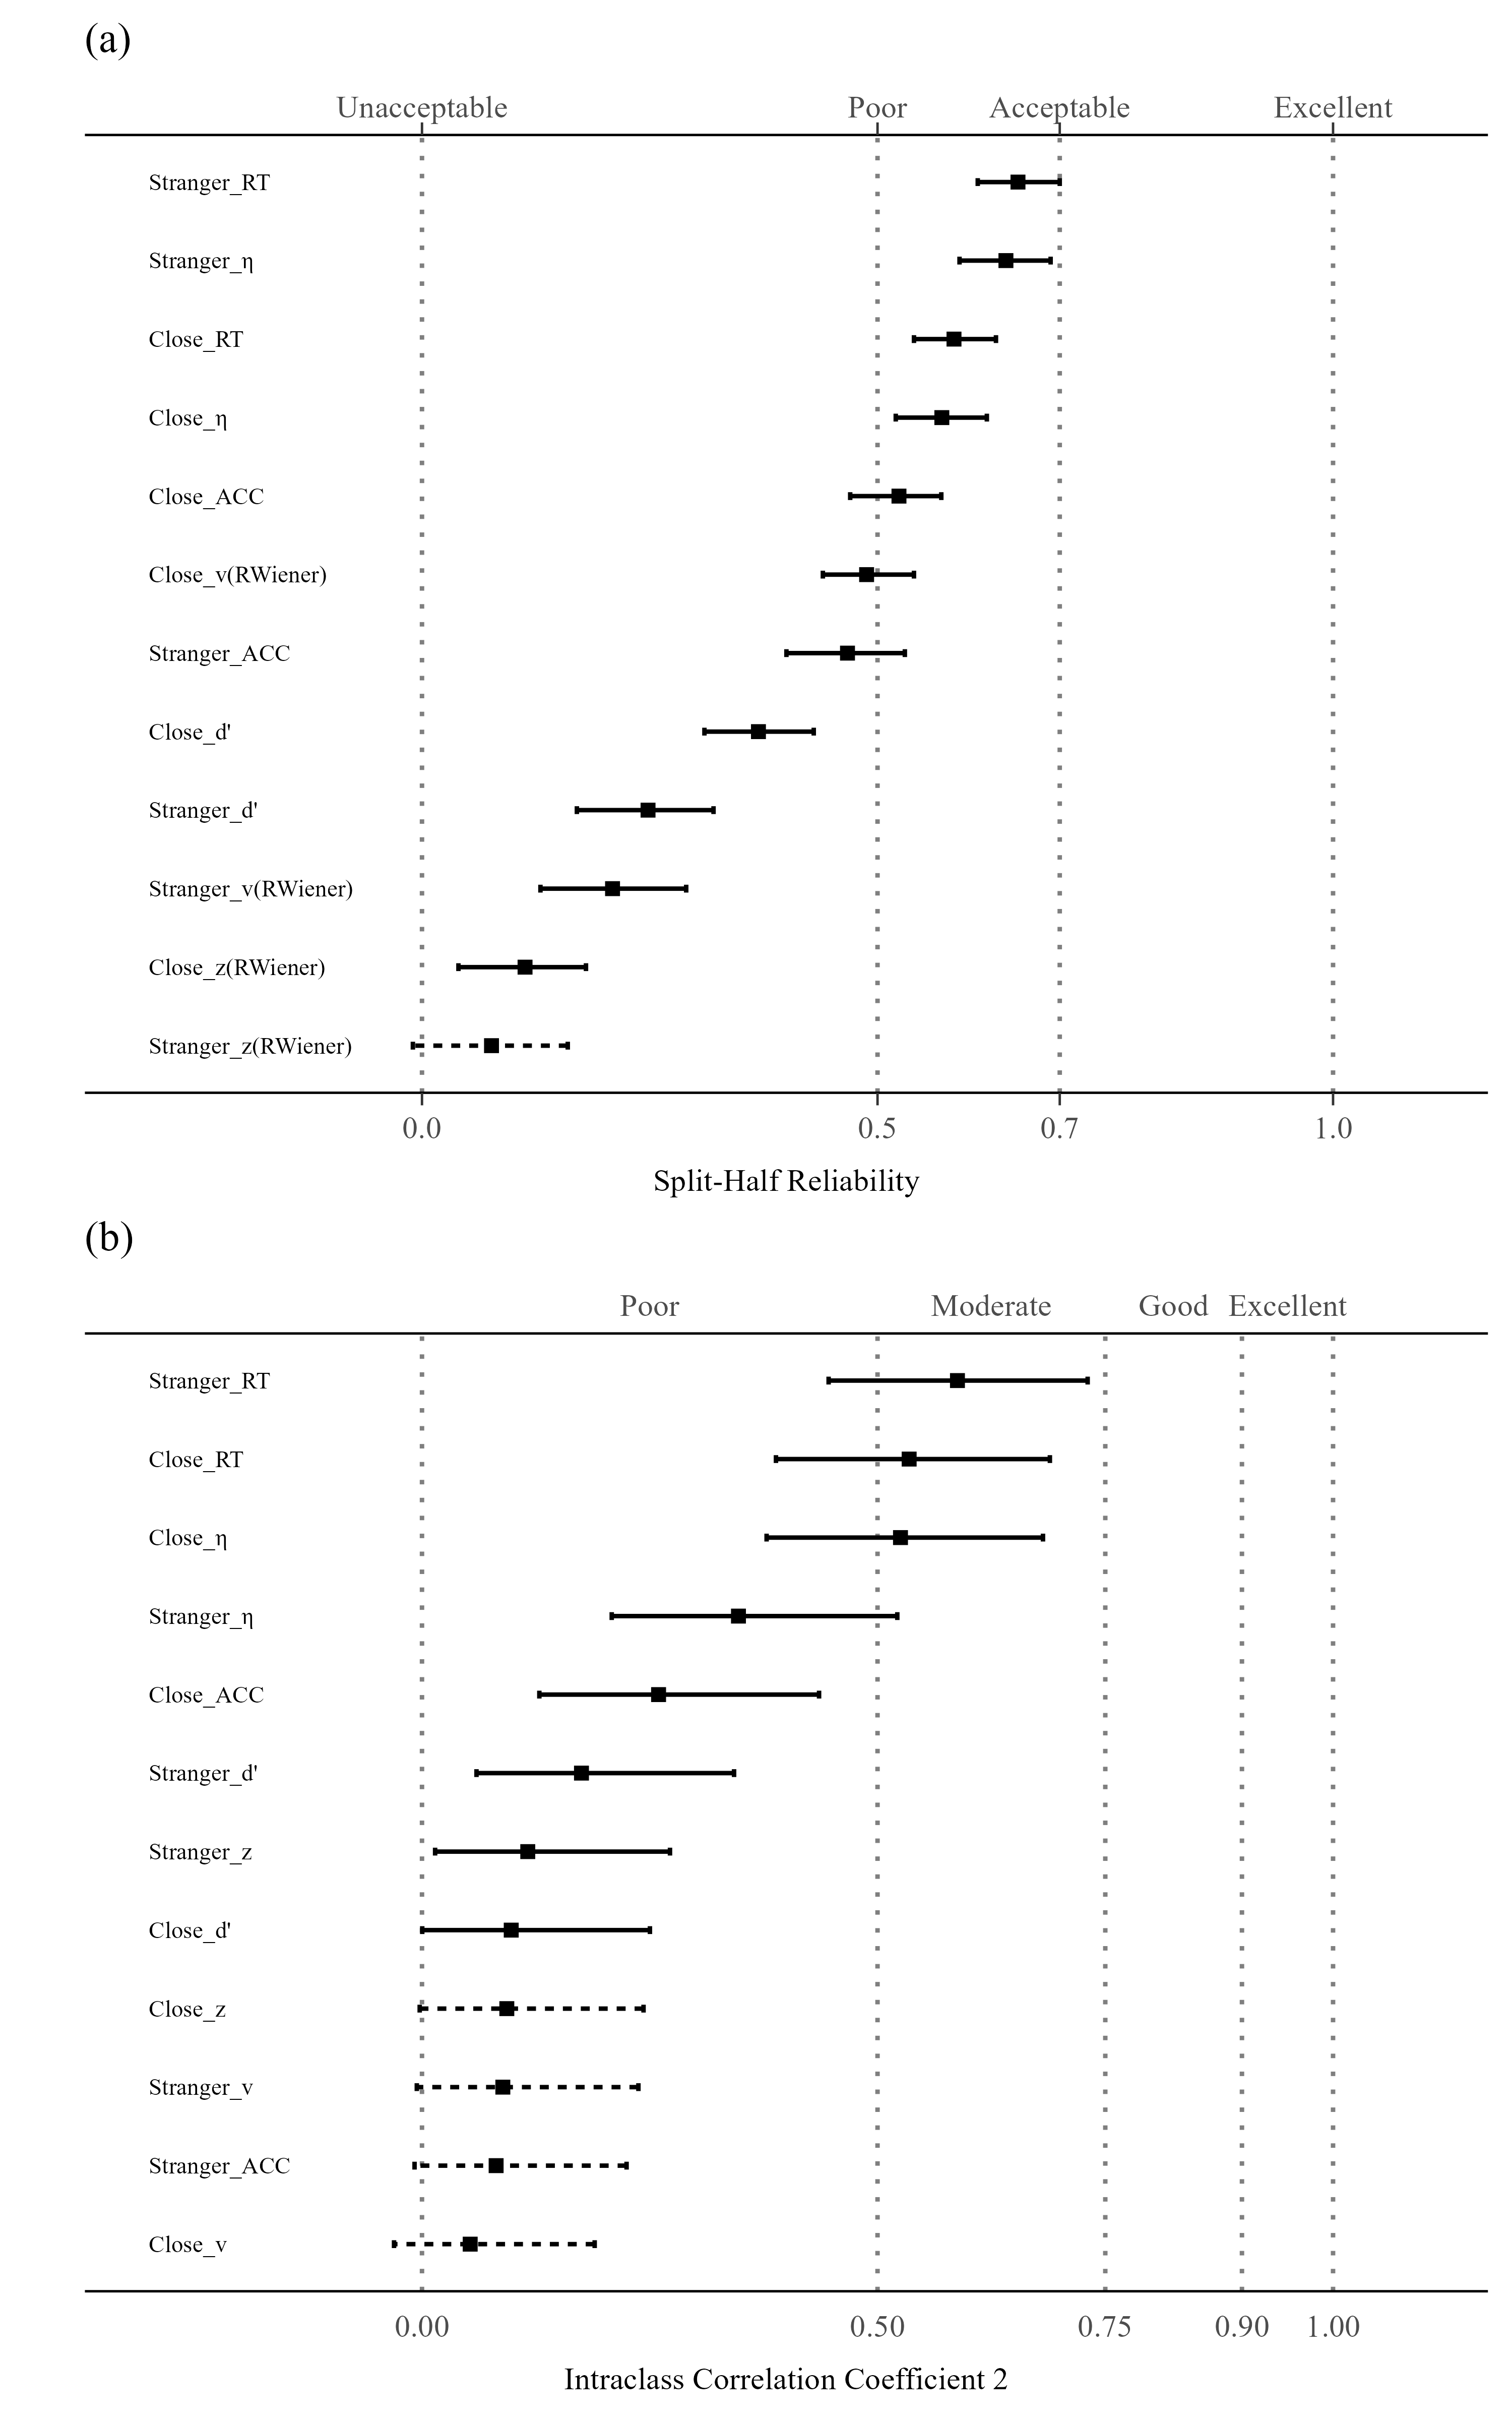
\includegraphics[width=1\textwidth]{./Figure/Fig_4_shr_icc.png}
	\caption{ Reliability for Different SPE Measures. (a) The Weighted Average Split-Half Reliability (Monte-Carlo); (b) Intraclass Correlation Coefficient (ICC2). \textit{Note}: The vertical axis represents 12 different SPE measures, combining six indicators (RT, ACC, $d'$, $\eta$, \textit{v}, \textit{z}) and two baseline conditions (``Close other" and ``Stranger"). The weighted average split-half reliability (figure a) and ICC values and their corresponding 95\% confidence intervals are illustrated using points and lines. The dashed line indicates that the confidence interval for that point estimate extends across 0, implying a non-significant value. Due to the fact that there is only one paper for ``Celebrity" and one for ``Nonperson", their results is presented in the supplementary materials.
	}
	\label{fig:shr_icc}
\end{figure}

We found that, among all SPE measures, the four with highest split-half reliabilities were as follows: Reaction Time (RT) with ``Stranger" as baseline ($r = .65, SE = .02, p <.001, 95\% $CI [.61, .70]); Efficiency ($\eta$) with ``Stranger" as baseline ($r = .64, SE  = .03, 95\% $CI [.59, .69]); RT with ``Close other" as baseline ($r = .58, SE = .02, 95\% $CI [.54, .63]); $\eta$ with ``Close other" as baseline ($r = .57, SE = .02, 95\% $ CI [.52, . 62]). These SPE measures achieved a split-half reliability around 0.6 or higher, which is considered acceptable. For all other SPE measures, the reliability was around 0.5 or lower, indicating poor reliability. These included Accuracy (ACC), Sensitivity Score ($d'$), Drift Rate (\textit{v}), and Starting Point (\textit{z}) under four baselines. It's worth noting that split-half reliability of \textit{z}, starting point parameter estimated from DDM, for all baselines were around 0, which suggested a total lack of reliability.


\subsection{Test-retest Reliability}\label{subsec:testretest}

ICC could only be calculated for dataset from our labortory \parencite{hu2023data}, which has 2 baseline conditions, the ``Close other” and ``Stranger”, in the experimental design. The ICC2, which measures the reliability for individual differences, aligns with the findings observed in split-half reliability estimation (see Fig. \ref{fig:shr_icc}(b)). Specifically, when using ``Close other” as baseline, the ICC2 for SPE measured by RT was .53 ($95\%$ CI [.39, .69]), and for Efficiency, it was .52 ($95\%$ CI [.38, .68]). Meanwhile, when ``Stranger" was used as baseline, the ICC2 for RT was .58 ($95\%$ CI [.45, .73]), and for Efficiency, it was .35 ($95\%$ CI [.21, .52]). All other measures of SPE exhibited reliability lower than 0.5. To test the robustness of the results, we explored one additional datasets that included re-test session but deviated strongly from the original SPMT, the result showed similar pattern here (see Supplementary Fig. S5).
\clearpage

\section{Discussion}\label{sec5}

In this pre-registered study, we examined the reliability of various measures from the Self Perceptual Matching Task (SPMT) in assessing the self-prioritization effect (SPE) using a multiverse approach. Our analyses revealed that, except parameters \textit{z} from DDM, all the other measures exhibited robust SPE. However, when it came to the reliability, only two measures of SPE, Reaction Time and Efficiency, exhibited acceptable to moderate reliability, among all indicators that has been reported in the literature. Our results suggested that the current implementation of SPMT was not well-suited for assessing individual differences. Taken together, our study revealed a ``reliability paradox" of SPE as measured by SPMT. These findings provided important methodological insights to future studies of SPE.

First, the Reaction Time (RT) and Efficiency ($\eta$) appeared to be the best measures among all different ways to measure SPE (the other were ACC, $d'$, parameter \textit{v} and \textit{z} from DDM). Our results revealed that the Reaction Time and Efficiency performed relatively well on both group-level and individual-level. On group level, effect sizes of SPE as measured by Reaction Time and Efficiency were moderate to large effect; on individual-level, SPE as measured by Reaction Time and Efficiency were higher for both split-half and test-retest reliability than other measures of SPE. Moreover, for different baseline conditions used for calculating SPE in the literature, ``Stranger” and ``Close other” (e.g., friends, or mother) are the most commonly utilized. Notably, ``Stranger” produced slightly higher effect size for most of the six indicators and demonstrated greater reliability when it came to Reaction Time. Therefore, for researchers interested in balancing between the group-level SPE and reliability, using Reaction Time and Efficiency as the indicators might be a good choice. 

Second, taken the group-level robustness and individual-level results together, our findings revealed a ``reliability paradox” in SPMT. We observed that the majority of the SPE measures demonstrated moderate to large effect sizes when analyzed at the group level. However, when considering individual differences, only the SPE measures derived from RT and Efficiency displayed comparatively higher values than other SPE measures but still did not meet the criteria for a satisfactory split-half reliability. Likewise, when examining the reliability across multiple time points using ICC2, RT and Efficiency still ranked the highest but only showed moderate levels of test-retest reliability. Our finding also aligned with the “reliability paradox” of cognitive tasks discovered in previous studies \parencite{hedge2018reliability,enkavi2019large}. The precise causes behind the reliability paradox observed in SPE measurements using the SPMT warrant thorough investigation. However, one of the most plausible explanations is that the SPMT, like other cognitive tasks, tends to exhibit minimal variability among participants while maximizing the detection of SPE at the group level \parencite{liljequist2019intraclass}. Consequently, this reliability paradox sheds light on the specific types of inquiries that the SPMT can proficiently address and those it cannot.

More specifically, the relatively low reliability of all the SPE measures calls for attention when researchers are interested in measuring individual differences, such as in clinical settings \parencite[e.g.,] []{karvelis2023individual}, or searching an association with data from questionnaires \parencite{hedge2018reliability}). As the SPMT was designed to achieve robust group-level SPE rather than to measure individual differences, researchers need to re-design the task if they are interested in assessing individual difference. Recently, researchers have proposed several ways to enhance the reliability of cognitive task, such as gamification \parencite{friehs2020effective}, using latent model \parencite{enkavi2019large, eisenberg2019uncovering} or generative models \parencite{haines2020theoretically} to analyze the data . Some of these suggestions has already been validated by empirical data. For example, \textcite{kucina2023calibration} re-designed cognitive conflict task by incorporating more trials and gamification indeed improved the reliability as compared to traditional Stroop task alone. Our exploratory analyses of the relationship between trial numbers and reliability also suggest that increasing trials numbers may improve reliability (please refer to the Supplementary section 2.4). 

Finally,a uprising result is the notably low split-half and test-retest reliability observed in the parameters (\textit{v} and \textit{z}) derived from the Drift-Diffusion Model. In our analyses, we applied common and easy-to-use methods to datasets that included at least 60 trials, and estimated parameters for each condition of each participant and then calculated the reliability. The reliability of both the drift rate (\textit{v}) and the starting point (\textit{z}) fell well below acceptable levels. These findings raised concerns about applying the standard drift-diffusion to data from SPMT directly. Previous studies found that standard drift-diffusion model did not fit the data from matching task \parencite{groulx2020ez}. Similarly, \textcite{schaaf2023test} recently found poor reliability for the parameter estimates of the standard reinforcement learning model in cognitive tasks. These findings called for a more principled approach when modeling behavioral data to more accurately capture the fundamental cognitive processes at play \parencite[e.g.,][]{wilson2019ten}, instead of applying the standard DDM blindly.  


\subsection{Implications of the Current Study}\label{subsec:impl}
Our findings can offer an initial guide for researchers considering the use of SPMT. Firstly, we recommend that researchers employ Reaction time and Efficiency as the indicators of SPE since they strike a balance between achieving a substantial effect size at the group level and ensuring reliability at the individual level. Second, if researchers are interested in relatively bigger group-level effect size, using the ``Self vs Stranger" contrast may prove beneficial. Third, if feasible, increasing the number of trials, as it may enhance the overall reliability of the measurements. Lastly, we caution against the careless application of the standard drift-diffusion model and instead advocate for a principled modeling approach.

\subsection{Limitations}\label{subsec:lim}
Several limitations warrant acknowledgment. Firstly, although we made efforts to enhance sample diversity by including open data when available, it is important to note that the majority of our samples still consisted of individuals from what is commonly referred to as ``(W)EIRD" populations \parencite{rad2018toward,yue2023weird}, most of the participants were recruited from universities and are healthy adults. As a result, our findings may not be fully representative of the broader population, and it is necessary to include a more diverse sample to ensure greater generalizability of the paradigm. Secondly, our results reported here assessed the robustness and reliability of SPE with the original experimental design of \textcite{sui2012perceptual}, which means the robustness and reliability of different variants of SPMT still need further investigation. For a more systematical meta-analysis of SPE measured by SPMT, please see our on-going project (\url{https://osf.io/euqmf}). Thirdly, when assessing the intraclass correlation coefficients (ICC2), only one dataset had available  data from multiple tests, which could potentially limit the representativeness of the results. This issue is mitigated by the fact that additional analysis of one datasets (see supplementary section 2.3) that with different design showed similar results as we reported in the main text. 

\section{Conclusion}\label{sec13}

This study provided an empirical assessment of the reliability of the self-perceptual matching task (SPMT). We found a robust self-prioritization effect for Reaction Time and Efficiency. Mean while, the reliability of the most robust SPE measure fell short of being satisfactory. The results of the current study may serve as a bench marker for the improvement of future studies.

\section*{Acknowledgments}

The authors declare that this research received no external funding.

\section*{Author Contributions}

HCP contributed to the conception and supervision of the study. HCP contributed to data collection. LZ, ZYR and HMZ wrote the simulation code for pre-registration. HMZ collected the datasets from published papers and performed data pre-processing, analysis and visualize the results. LZ, HMZ and HCP contributed to discussing the results and the drafting of the final manuscript. HCP, JS, LZ and HMZ critically revised the manuscript.

\section*{Data and Material Availability}

The pre-registration plan is available at OSF( \url{https://osf.io/zv628}). The de-identified raw data from our lab is available at Science Data Bank (\url{https://doi.org/10.57760/sciencedb.08117}). The simulated data is accessible on GitHub (\url{https://github.com/Chuan-Peng-Lab/ReliabilitySPE}). 

\section*{Code Availability}

Code used to simulate and analyze the data is made accessible on GitHub (\url{https://github.com/Chuan-Peng-Lab/ReliabilitySPE}). 

\section*{Competing Interests}

The authors declare no competing interests.



%%===========================================================================================%%
%% If you are submitting to one of the Nature Portfolio journals, using the eJP submission   %%
%% system, please include the references within the manuscript file itself. You may do this  %%
%% by copying the reference list from your .bbl file, paste it into the main manuscript .tex %%
%% file, and delete the associated \verb+\bibliography+ commands.                            %%
%%===========================================================================================%%


\printbibliography
%\bibliography{sn-bibliography}% common bib file
%% if required, the content of .bbl file can be included here once bbl is generated
%%\input sn-article.bbl
\end{document}
